\documentclass[12pt,oneside]{book}

%%%%%%%%%%%%%%%%%%%%%%%%%%%%%%%%%%%%%%%%%%%%%%%%%%%%%%%%%%%%%%%%%%%%%%%%%%%%%%%%%%%%%%%%%%%%%%%%%%%
%                                                                                                 %
% The mathematical style of these documents follows                                               %
%                                                                                                 %
% A. Thompson and B.N. Taylor. The NIST Guide for the Use of the International System of Units.   %
%    NIST Special Publication 881, 2008.                                                          %
%                                                                                                 %
% http://www.nist.gov/pml/pubs/sp811/index.cfm                                                    %
%                                                                                                 %
%%%%%%%%%%%%%%%%%%%%%%%%%%%%%%%%%%%%%%%%%%%%%%%%%%%%%%%%%%%%%%%%%%%%%%%%%%%%%%%%%%%%%%%%%%%%%%%%%%%

% $Date: 2013-11-26 10:43:59 -0500 (Tue, 26 Nov 2013) $
% $Revision: 17538 $
% $Author: gforney $

%%%%%%%%%%%%%%%%%%%%%%%%%%%%%%%%%%%%%%%%%%%%%%%%%%%%%%%%%%%%%%%%%%%%%%%%%%%%%%%%%%%%%%%%%%%%%%%%%%%
%                                                                                                 %
% The mathematical style of these documents follows                                               %
%                                                                                                 %
% A. Thompson and B.N. Taylor. The NIST Guide for the Use of the International System of Units.   %
%    NIST Special Publication 881, 2008.                                                          %
%                                                                                                 %
% http://www.nist.gov/pml/pubs/sp811/index.cfm                                                    %
%                                                                                                 %
%%%%%%%%%%%%%%%%%%%%%%%%%%%%%%%%%%%%%%%%%%%%%%%%%%%%%%%%%%%%%%%%%%%%%%%%%%%%%%%%%%%%%%%%%%%%%%%%%%%

% Packages which force the use of better TeX coding
% Mostly from http://tex.stackexchange.com/q/19264
%%\RequirePackage[l2tabu, orthodox]{nag}
%%\usepackage{fixltx2e}
%\usepackage{isomath} % Disabled for the moment because it changes the syntax for bold and roman Greek math symbols
%%\usepackage[all,warning]{onlyamsmath}
%\usepackage{strict} % Commented out for now because it is uncommon. A copy of style.sty is in Manuals/LaTeX_Style_Files/.

\usepackage{times,mathptmx}
\usepackage[pdftex]{graphicx}
\usepackage{tabularx,ragged2e,booktabs,caption}
\usepackage{multirow}
\usepackage{pdfsync}
\usepackage{tikz}
\usepackage{pgfplots}
%\pgfplotsset{compat=1.7}
\usepackage{tocloft}
\usepackage{color}
\usepackage{amsmath}
\definecolor{linknavy}{rgb}{0,0,0.50196}
\definecolor{linkred}{rgb}{1,0,0}
\definecolor{linkblue}{rgb}{0,0,1}
\usepackage{float}
\usepackage{caption}
\usepackage{graphpap}
\usepackage{rotating}
\usepackage{graphicx}
\usepackage{geometry}
\usepackage{relsize}
\usepackage{longtable}
\usepackage{lscape}
\usepackage{amssymb}
\usepackage{makeidx} % Create index at end of document
\usepackage[nottoc,notlof,notlot]{tocbibind} % Put the bibliography and index in the ToC
\usepackage{lastpage} % Automatic last page number reference.
\usepackage[T1]{fontenc}
\usepackage{enumerate}
\usepackage{upquote}
\usepackage{moreverb}
\usepackage{xfrac}
\usepackage{cite}

\newcommand{\nopart}{\expandafter\def\csname Parent-1\endcsname{}} % To fix table of contents in pdf.
\newcommand{\ct}{\tt\small} % eventually will be deprecated due to http://www.tex.ac.uk/cgi-bin/texfaq2html?label=2letterfontcmd
\newcommand{\textct}[1]{\texttt{\small #1}}

\usepackage{tocstyle} % Fix table of contents sections from overlapping section titles
\usetocstyle{standard}
\usepackage{siunitx}
\sisetup{
    detect-all = true,
    input-decimal-markers = {.},
    input-ignore = {,},
    inter-unit-product = \ensuremath{{}\cdot{}},
    multi-part-units = repeat,
    number-unit-product = \text{~},
    per-mode = fraction,
    separate-uncertainty = true,
}

\usepackage{listings}
\usepackage{textcomp}
\definecolor{lbcolor}{rgb}{0.96,0.96,0.96}
\lstset{
    %backgroundcolor=\color{lbcolor},
    tabsize=4,
    rulecolor=,
    language=Fortran,
        basicstyle=\footnotesize\ttfamily,
        upquote=true,
        aboveskip={\baselineskip},
        belowskip={\baselineskip},
        columns=fixed,
        extendedchars=true,
        breaklines=true,
        breakatwhitespace=true,
        frame=none,
        showtabs=false,
        showspaces=false,
        showstringspaces=false,
        identifierstyle=\ttfamily,
        keywordstyle=\color[rgb]{0,0,0},
        commentstyle=\color[rgb]{0,0,0},
        stringstyle=\color[rgb]{0,0,0},
}

\usepackage[pdftex,
        colorlinks=true,
        urlcolor=linkblue,     % \href{...}{...} external (URL)
        citecolor=linkred,     % citation number colors
        linkcolor=linknavy,    % \ref{...} and \pageref{...}
        pdfproducer={pdflatex},
        pdfpagemode=UseNone,
        bookmarksopen=true,
        plainpages=false,
        verbose]{hyperref}

% The Following commented code makes the ``Draft'' watermark on each page.
%\usepackage{eso-pic}
%\usepackage{type1cm}
%\makeatletter
%   \AddToShipoutPicture{
%     \setlength{\@tempdimb}{.5\paperwidth}
%     \setlength{\@tempdimc}{.5\paperheight}
%     \setlength{\unitlength}{1pt}
%     \put(\strip@pt\@tempdimb,\strip@pt\@tempdimc){
%     \makebox(0,0){\rotatebox{45}{\textcolor[gray]{0.75}{\fontsize{8cm}\selectfont{RC6}}}}}
% }
%\makeatother

\setlength{\textwidth}{6.5in}
\setlength{\textheight}{9.0in}
\setlength{\topmargin}{0.in}
\setlength{\headheight}{0.pt}
\setlength{\headsep}{0.in}
\setlength{\parindent}{0.25in}
\setlength{\oddsidemargin}{0.0in}
\setlength{\evensidemargin}{0.0in}
\setlength{\leftmargini}{\parindent} % Controls the indenting of the "bullets" in a list
\setlength{\cftsecnumwidth}{0.45in}
\setlength{\cftsubsecnumwidth}{0.5in}
\setlength{\cftfignumwidth}{0.45in}
\setlength{\cfttabnumwidth}{0.45in}

\newcommand{\titlesigs}
{
\small
\flushright{U.S. Department of Commerce \\
{\em Penny Pritzker, Secretary} \\
\hspace{1in} \\
National Institute of Standards and Technology \\
{\em Willie May, Under Secretary of Commerce for Standards and Technology and Acting Director} }
}

% commands to use for "official" cover and title pages
% see smokeview verification guide to see how they are used

\newcommand{\headerA}[1]{
\flushright{
\fontsize{20}{24}\selectfont
\bf{NIST Special Publication #1}}
}

\newcommand{\headerB}[1]{
\flushright{
\fontsize{28}{33.6}\selectfont
\bf{#1}
}
}

\newcommand{\headerC}[1]{
\vspace{.5in}
\flushright{\fontsize{14}{16.8}\selectfont
#1}
}

\frenchspacing

\newcommand{\dod}[2]{\frac{\partial #1}{\partial #2}}
\newcommand{\DoD}[2]{\frac{\mathrm{D} #1}{\mathrm{D} #2}}
\newcommand{\dsods}[2]{\frac{\partial^2 #1}{\partial #2^2}}
\renewcommand{\d}{\,\mathrm{d}}
\newcommand{\dx}{\delta x}
\newcommand{\dy}{\delta y}
\newcommand{\dz}{\delta z}
\newcommand{\degF}{$^\circ$F}
\newcommand{\degC}{$^\circ$C}
\newcommand{\x}{x}
\newcommand{\y}{y}
\newcommand{\z}{z}
\newcommand{\dt}{\delta t}
\newcommand{\dn}{\delta n}
\newcommand{\cH}{H}
\newcommand{\hu}{u}
\newcommand{\hv}{v}
\newcommand{\hw}{w}
\newcommand{\la}{\lambda}
\newcommand{\bO}{{\Omega}}
\newcommand{\bo}{{\mathbf{\omega}}}
\newcommand{\btau}{\mathbf{\tau}}
\newcommand{\bdelta}{{\mathbf{\delta}}}
\newcommand{\sumyw}{\sum (Y_\alpha/W_\alpha)}
\newcommand{\oW}{\overline{W}}
\newcommand{\om}{\ensuremath{\omega}}
\newcommand{\omx}{\omega_x}
\newcommand{\omy}{\omega_y}
\newcommand{\omz}{\omega_z}
\newcommand{\erf}{\hbox{erf}}
\newcommand{\erfc}{\hbox{erfc}}
\newcommand{\bF}{{\mathbf{F}}}
\newcommand{\bG}{{\mathbf{G}}}
\newcommand{\bof}{{\mathbf{f}}}
\newcommand{\bq}{{\mathbf{q}}}
\newcommand{\br}{{\mathbf{r}}}
\newcommand{\bu}{{\mathbf{u}}}
\newcommand{\bx}{{\mathbf{x}}}
\newcommand{\bk}{{\mathbf{k}}}
\newcommand{\bv}{{\mathbf{v}}}
\newcommand{\bg}{{\mathbf{g}}}
\newcommand{\bn}{{\mathbf{n}}}
\newcommand{\bS}{{\mathbf{S}}}
\newcommand{\bW}{\overline{W}}
\newcommand{\dS}{d{\mathbf{S}}}
\newcommand{\bs}{{\mathbf{s}}}
\newcommand{\bI}{{\mathbf{I}}}
\newcommand{\hp}{H}
\newcommand{\trho}{\tilde{\rho}}
\newcommand{\dph}{{\delta\phi}}
\newcommand{\dth}{{\delta\theta}}
\newcommand{\tp}{\tilde{p}}
\newcommand{\bp}{\overline{p}}
\newcommand{\dQ}{\dot{Q}}
\newcommand{\dq}{\dot{q}}
\newcommand{\dbq}{\dot{\mathbf{q}}}
\newcommand{\dm}{\dot{m}}
\newcommand{\ha}{\frac{1}{2}}
\newcommand{\ft}{\frac{4}{3}}
\newcommand{\ot}{\frac{1}{3}}
\newcommand{\fofi}{\frac{4}{5}}
\newcommand{\of}{\frac{1}{4}}
\newcommand{\twth}{\frac{2}{3}}
\newcommand{\R}{R}
\newcommand{\be}{\begin{equation}}
\newcommand{\ee}{\end{equation}}
\newcommand{\RE}{\hbox{Re}}
\newcommand{\LE}{\hbox{Le}}
\newcommand{\PR}{\hbox{Pr}}
\newcommand{\PE}{\hbox{Pe}}
\newcommand{\NU}{\hbox{Nu}}
\newcommand{\SC}{\hbox{Sc}}
\newcommand{\SH}{\hbox{Sh}}
\newcommand{\WE}{\hbox{We}}
\newcommand{\COTWO}{\text{\tiny \hbox{CO}$_2$}}
\newcommand{\HTWOO}{\text{\tiny \hbox{H}$_2$\hbox{O}}}
\newcommand{\OTWO}{\text{\tiny \hbox{O}$_2$}}
\newcommand{\NTWO}{\text{\tiny \hbox{N}$_2$}}
\newcommand{\CO}{\text{\tiny \hbox{CO}}}
\newcommand{\F}{\text{\tiny \hbox{F}}}
\newcommand{\C}{\text{\tiny \hbox{C}}}
\newcommand{\Hy}{\text{\tiny \hbox{H}}}
\newcommand{\So}{\text{\tiny \hbox{S}}}
\newcommand{\M}{\text{\tiny \hbox{M}}}
\newcommand{\xx}{\text{\tiny \hbox{x}}}
\newcommand{\yy}{\text{\tiny \hbox{y}}}
\newcommand{\zz}{\text{\tiny \hbox{z}}}
\newcommand{\smvlines}{115~000}

\newcommand{\calH}{\mathcal{H}}
\newcommand{\calR}{\mathcal{R}}

\newcommand{\dif}{\mathrm{d}}
\newcommand{\Div}{\nabla\cdot}
\newcommand{\D}{\mbox{D}}
\newcommand{\mhalf}{\mbox{$\frac{1}{2}$}}
\newcommand{\thalf}{\mbox{\tiny $\frac{1}{2}$}}
\newcommand{\tripleprime}{{\prime\prime\prime}}
\newcommand{\ppp}{{\prime\prime\prime}}
\newcommand{\pp}{{\prime\prime}}

\newcommand{\superscript}[1]{\ensuremath{^{\textrm{\tiny #1}}}}
\newcommand{\subscript}[1]{\ensuremath{_{\textrm{\tiny #1}}}}

\newcommand{\rb}[1]{\raisebox{1.5ex}[0pt]{#1}}

\newcommand{\Ra}{$\Rightarrow$}
\newcommand{\hhref}[1]{\href{#1}{{\tt #1}}}
\newcommand{\fdsinput}[1]{{\scriptsize\verbatiminput{../../Verification/Visualization/#1}}}

\definecolor{AQUAMARINE}{rgb}{0.49804,1.00000,0.83137}
\definecolor{ANTIQUE WHITE}{rgb}{0.98039,0.92157,0.84314}
\definecolor{BEIGE}{rgb}{0.96078,0.96078,0.86275}
\definecolor{BLACK}{rgb}{0.00000,0.00000,0.00000}
\definecolor{BLUE}{rgb}{0.00000,0.00000,1.00000}
\definecolor{BLUE VIOLET}{rgb}{0.54118,0.16863,0.88627}
\definecolor{BRICK}{rgb}{0.61176,0.40000,0.12157}
\definecolor{BROWN}{rgb}{0.64706,0.16471,0.16471}
\definecolor{BURNT SIENNA}{rgb}{0.54118,0.21176,0.05882}
\definecolor{BURNT UMBER}{rgb}{0.54118,0.20000,0.14118}
\definecolor{CADET BLUE}{rgb}{0.37255,0.61961,0.62745}
\definecolor{CHOCOLATE}{rgb}{0.82353,0.41176,0.11765}
\definecolor{COBALT}{rgb}{0.23922,0.34902,0.67059}
\definecolor{CORAL}{rgb}{1.00000,0.49804,0.31373}
\definecolor{CYAN}{rgb}{0.00000,1.00000,1.00000}
\definecolor{DIMGRAY }{rgb}{0.41176,0.41176,0.41176}
\definecolor{EMERALD GREEN}{rgb}{0.00000,0.78824,0.34118}
\definecolor{FIREBRICK}{rgb}{0.69804,0.13333,0.13333}
\definecolor{FLESH}{rgb}{1.00000,0.49020,0.25098}
\definecolor{FOREST GREEN}{rgb}{0.13333,0.54510,0.13333}
\definecolor{GOLD }{rgb}{1.00000,0.84314,0.00000}
\definecolor{GOLDENROD}{rgb}{0.85490,0.64706,0.12549}
\definecolor{GRAY}{rgb}{0.50196,0.50196,0.50196}
\definecolor{GREEN}{rgb}{0.00000,1.00000,0.00000}
\definecolor{GREEN YELLOW}{rgb}{0.67843,1.00000,0.18431}
\definecolor{HONEYDEW}{rgb}{0.94118,1.00000,0.94118}
\definecolor{HOT PINK}{rgb}{1.00000,0.41176,0.70588}
\definecolor{INDIAN RED}{rgb}{0.80392,0.36078,0.36078}
\definecolor{INDIGO}{rgb}{0.29412,0.00000,0.50980}
\definecolor{IVORY}{rgb}{1.00000,1.00000,0.94118}
\definecolor{IVORY BLACK}{rgb}{0.16078,0.14118,0.12941}
\definecolor{KELLY GREEN}{rgb}{0.00000,0.50196,0.00000}
\definecolor{KHAKI}{rgb}{0.94118,0.90196,0.54902}
\definecolor{LAVENDER}{rgb}{0.90196,0.90196,0.98039}
\definecolor{LIME GREEN}{rgb}{0.19608,0.80392,0.19608}
\definecolor{MAGENTA}{rgb}{1.00000,0.00000,1.00000}
\definecolor{MAROON}{rgb}{0.50196,0.00000,0.00000}
\definecolor{MELON}{rgb}{0.89020,0.65882,0.41176}
\definecolor{MIDNIGHT BLUE}{rgb}{0.09804,0.09804,0.43922}
\definecolor{MINT}{rgb}{0.74118,0.98824,0.78824}
\definecolor{NAVY}{rgb}{0.00000,0.00000,0.50196}
\definecolor{OLIVE}{rgb}{0.50196,0.50196,0.00000}
\definecolor{OLIVE DRAB}{rgb}{0.41961,0.55686,0.13725}
\definecolor{ORANGE}{rgb}{1.00000,0.50196,0.00000}
\definecolor{ORANGE RED}{rgb}{1.00000,0.27059,0.00000}
\definecolor{ORCHID}{rgb}{0.85490,0.43922,0.83922}
\definecolor{PINK}{rgb}{1.00000,0.75294,0.79608}
\definecolor{POWDER BLUE}{rgb}{0.69020,0.87843,0.90196}
\definecolor{PURPLE}{rgb}{0.50196,0.00000,0.50196}
\definecolor{RASPBERRY}{rgb}{0.52941,0.14902,0.34118}
\definecolor{RED}{rgb}{1.00000,0.00000,0.00000}
\definecolor{ROYAL BLUE}{rgb}{0.25490,0.41176,0.88235}
\definecolor{SALMON}{rgb}{0.98039,0.50196,0.44706}
\definecolor{SANDY BROWN}{rgb}{0.95686,0.64314,0.37647}
\definecolor{SEA GREEN}{rgb}{0.32941,1.00000,0.62353}
\definecolor{SEPIA}{rgb}{0.36863,0.14902,0.07059}
\definecolor{SIENNA}{rgb}{0.62745,0.32157,0.17647}
\definecolor{SILVER}{rgb}{0.75294,0.75294,0.75294}
\definecolor{SKY BLUE}{rgb}{0.52941,0.80784,0.92157}
\definecolor{SLATEBLUE}{rgb}{0.41569,0.35294,0.80392}
\definecolor{SLATE GRAY}{rgb}{0.43922,0.50196,0.56471}
\definecolor{SPRING GREEN}{rgb}{0.00000,1.00000,0.49804}
\definecolor{STEEL BLUE}{rgb}{0.27451,0.50980,0.70588}
\definecolor{TAN}{rgb}{0.82353,0.70588,0.54902}
\definecolor{TEAL}{rgb}{0.00000,0.50196,0.50196}
\definecolor{THISTLE}{rgb}{0.84706,0.74902,0.84706}
\definecolor{TOMATO }{rgb}{1.00000,0.38824,0.27843}
\definecolor{TURQUOISE}{rgb}{0.25098,0.87843,0.81569}
\definecolor{VIOLET}{rgb}{0.93333,0.50980,0.93333}
\definecolor{VIOLET RED}{rgb}{0.81569,0.12549,0.56471}
\definecolor{WHITE}{rgb}{1.00000,1.00000,1.00000}
\definecolor{YELLOW}{rgb}{1.00000,1.00000,0.00000}

\pgfplotsset{
	colormap={blackwhite}{[5pt]
		rgb255(0pt)=(0,0,255); 
		rgb255(100pt)=(0,255,255); 
		rgb255(200pt)=(0,255,0); 
		rgb255(300pt)=(255,255,0); 
		rgb255(400pt)=(255,0,0)
	},
} % defines smokeview colorbar


\floatstyle{boxed}
\newfloat{notebox}{H}{lon}
\newfloat{warning}{H}{low}

% Set default longtable alignment
\setlength\LTleft{0pt}
\setlength\LTright{0pt}


% Rename chapter headings
\renewcommand{\chaptername}{Section}
\renewcommand{\bibname}{References}

% Math shortcuts
\renewcommand{\sb}[1]{_\mathrm{#1}}
\renewcommand{\C}{\mbox{C}}
\renewcommand{\H}{\mbox{H}}
\renewcommand{\O}{\mbox{O}}
\newcommand{\N}{\mbox{N}}

% Extra packages
\usepackage{xfrac}

\begin{document}

\bibliographystyle{unsrt}
\pagestyle{empty}

\begin{minipage}[t][9in][s]{6.25in}

\begin{flushright}
\fontsize{20}{24}\selectfont
\bf{NIST Technical Note XXXX}
\end{flushright}

\headerB{
Simulation of a Wind Driven \\
Basement Fire - \\
Riverdale Heights, MD \\
}

\normalsize

\headerC{
{
\flushright{
Craig G. Weinschenk \\
Kristopher J. Overholt \\
Daniel Madrzykowski \\

\vspace*{2\baselineskip}

\begingroup
\hypersetup{urlcolor=black}
\href{http://dx.doi.org/10.6028/NIST.TN.1838}{http://dx.doi.org/10.6028/NIST.TN.XXXX}
\endgroup
}

\vfill

\flushright{


\includegraphics[width=2.in]{../../../Bibliography/nistident_flright_vec} \\[.3in]
}
}
}

\end{minipage}

\newpage
\hspace{5in}
\newpage

\frontmatter

\pagenumbering{roman}

\begin{minipage}[t][9in][s]{6.25in}

\begin{flushright}
\fontsize{20}{24}\selectfont
\bf{NIST Technical Note XXXX}
\end{flushright}

\headerB{
Simulation of a Wind Driven \\
Basement Fire - \\
Riverdale Heights, MD \\
}

\headerC{
\flushright{
Craig G. Weinschenk \\
Kristopher J. Overholt \\
Daniel Madrzykowski \\
{\em Fire Research Division \\
Engineering Laboratory} \\

\vspace*{2\baselineskip}

\begingroup
\hypersetup{urlcolor=black}
\href{http://dx.doi.org/10.6028/NIST.TN.1838}{http://dx.doi.org/10.6028/NIST.TN.XXXX} \\
\endgroup

\vspace*{2\baselineskip}

August 2014}}

\vfill

\flushright{
\includegraphics[width=1in]{../../../Bibliography/doc} }

\titlesigs

\end{minipage}

\newpage

\begin{minipage}[t][9in][s]{6.25in}

\flushright{Certain commercial entities, equipment, or materials may be identified in this \\
document in order to describe an experimental procedure or concept adequately. \\
Such identification is not intended to imply recommendation or endorsement by the \\
National Institute of Standards and Technology, nor is it intended to imply that the \\
entities, materials, or equipment are necessarily the best available for the purpose. \\
}

\vspace{3in}

\large
\flushright{\bf National Institute of Standards and Technology Technical Note XXXX \\
Natl.~Inst.~Stand.~Technol.~Tech.~Note~XXXX, \pageref{LastPage} pages (August 2014) \\
% http://dx.doi.org/10.6028/NIST.TN.XXXX \\
CODEN: NTNOEF }

\vfill

\hspace{1in}

\end{minipage}

\newpage

\frontmatter

\pagestyle{plain}
\pagenumbering{roman}

\cleardoublepage
\phantomsection
\addcontentsline{toc}{chapter}{Contents}
\tableofcontents

\cleardoublepage
\phantomsection
\addcontentsline{toc}{chapter}{List of Figures}
\listoffigures

\cleardoublepage
\phantomsection
\addcontentsline{toc}{chapter}{List of Tables}
\listoftables

\chapter{List of Acronyms}

\begin{tabbing}
\hspace{1.5in} \= \\
EMS \> Emergency Medical Services \\
FDS \> Fire Dynamics Simulator \\
HGL \> Hot Gas Layer \\
HRR \> Heat Release Rate \\
HRRPUA \> Heat Release Rate per Unit Area \\
LODD \> Line of Duty Death \\
NIST \> National Institute of Standards and Technology \\
SFPE \> Society of Fire Protection Engineers \\
\end{tabbing}

\chapter{List of Symbols}

\begin{tabbing}
\hspace{1.5in} \= \\
ft \> foot \\
m \> meter \\
min \> minute \\
Pa \> Pascal \\
psi \> pound per square inch \\
s \> second \\
W \> Watt \\
$k$ \> thermal conductivity \\
$\rho$ \> density \\
$c_{p}$ \> specific heat \\
\end{tabbing}

\mainmatter

\chapter*{\centering Abstract}
\addcontentsline{toc}{chapter}{Abstract}

\chapter{Introduction}
Part of the function of the Fire Research Division at NIST is to develop and apply technology, measurements, and standards to improve the understanding of the behavior, prevention, and control of fires to enhance fire fighting operations and equipment, fire suppression, fire investigations, and disaster response. NIST has previously used the Fire Dynamics Simulator (FDS) fire model to provide insight into the fire development and thermal conditions of fires that have resulted in line of duty deaths (LODDs)~\cite{Madrzykowski:1,Iowa,Texas,Bryner:Charleston,barowy:texas}. The objective of these studies has been to improve the safety and effectiveness of firefighters.

On February 24, 2012, a fire in residential structure injured seven Prince George's County firefighters. NIST examined the fire dynamics of this incident at the request of the Prince George's Country Fire/Emergency Medical Services (EMS) Department. Computer simulations of the fire incident were conducted using the NIST Fire Dynamics Simulator~\cite{FDS_Users_Guide} and Smokeview~\cite{Smokeview_Users_Guide}  software to provide insight into the fire development and thermal conditions that likely existed in the residence during the fire. The specific objectives of the simulations detailed in this report are: 
\begin{enumerate}
\item To examine the effect of the flow path (including temperature, pressure, and fire conditions) in this multi-story residential structure using physics-based calculations.
\item To provide visualizations of the fire behavior that are representative of the conditions that members of the Prince George's Fire Department likely experienced during the course of their interior operations.
\end{enumerate}
This document describes the input and the results of the FDS (version 6.0.0) simulations. The simulations were developed using a combination of knowledge of the fire scenario and appropriate engineering approximations and assumptions. Analysis of the simulation results focuses on the hazardous conditions that developed following the development of a flow path inside of the structure. This document is organized as follows: Section~\ref{fire_sum} provides a summary of the fire incident, Section~\ref{model} describes the relevant model input parameters and assumptions that were used to develop the simulations, Section~\ref{results} presents the simulation results, and Section~\ref{discuss} discusses the simulation results as they relate to firefighter safety and effectiveness. Appendix~\ref{app_draw} contains dimensioned drawings of the first and second floor of the structure.


\chapter{Fire Incident Summary}
\label{fire_sum}
The account of events for this incident was documented by the Safety Investigation Team of the Prince George's County Fire/EMS Department~\cite{PGCounty2013}. At 21:11 hours on February 24, 2012 Prince George's Fire/EMS Department responded to a structure fire in Riverdale Heights, Maryland with a fire in the basement~\cite{PGCounty2013}. For the purpose of this analysis, the details regarding the timeline are considered to be approximate values. The following narrative of the incident, focused on the events which led to burn injuries to two emergency-personnel, was taken from the Prince George's County report~\cite{PGCounty2013}:
\begin{quote}
Truck 809 responded from quarters, as the first due truck company, and arrived on 57$^{th}$ Avenue right behind Engine 807B. When Truck 809 stopped to let Engine 807B layout, Truck 809 Can dismounted the truck and had to walk up the street as it pulled away. Truck 809 Officer observed a lot of smoke moving extremely fast through the front yard and across the street upon exiting the truck. Truck 809 Officer and Truck 809 Forcible Entry proceeded directly to the front door \ldots of the structure. Both of them entered the structure with full PPE, including SCBA, but without the protection of a hose line. Truck 809 Officer and Truck 809 Forcible Entry began primary searches on the first floor. At some point during the primary search, as conditions worsened, the front door closed, trapping Truck 809 Officer and Truck 809 Forcible Entry inside the structure. This situation could not have occurred if a charged hose line was operating inside the structure at the time the door slammed shut. They were the only firefighters operating on the first floor at that time. 

Truck 809 Forcible Entry was too large in physical stature to fit through the small window opening that he found on [the front of the structure]. Truck 809 Forcible Entry was unable to self-evacuate, and remained trapped inside. Due to rapidly deteriorating conditions, Truck 809 Officer was forced to self-rescue through another small window on [the front of the structure]. 

After exiting the structure, Truck 809 Officer screamed (to those on the exterior) that a firefighter was trapped inside. Truck 809 Officer then proceeded to the front door \ldots in an attempt to search for and rescue Truck 809 Forcible Entry, who was trapped inside. At this point multiple firefighters on the exterior assisted Truck 809 Officer in the search, rescue, and removal of Truck 809 Forcible Entry. Both Truck 809 Officer and Truck 809 Forcible Entry sustained serious injuries and were transported to MedStar/Washington Hospital Center. 

While the interior operations were occurring, Truck 809 Driver and Truck 809 Hook/Ladders were on the exterior throwing ladders to the structure. Truck 809 Hook/Ladders threw two ladders [front and left side], while Truck 809 Driver threw one ladder ([front side]). 
\end{quote}  

\noindent Table~\ref{tab:fire_info} shows an overview of the timeline of events.
\begin{table}[!h]
\centering
\captionof{table}[Abridged approximate fire event timeline]{Abridged Prince George's Fire/EMS approximate fire event timeline~\cite{PGCounty2013}}\label{tab:fire_info}
\begin{tabular}{cl}
\toprule[1.5pt]
Incident Time              &  Fire Behavior / Fireground Operation  \\
{[hh:mm:ss]}               &                                                               \\
\midrule
21:08:26   & First 911 call is made. \\[.25cm]
\multirow{3}{*}{21:11:03}  &   \multirow{3}{*}{\parbox{10cm} {Dispatch for a ``box'' alarm assignment- four engine companies, two truck companies, one rescue squad, and a commanding officer.}}    \\
                           &         \\
                           &         \\[.25cm]
21:12:55  &  First unit (Engine 807B) arrived on-scene.  \\[.25cm]
21:13:44  & Volunteer Chief 809A establishes incident command (IC).   \\[.25cm]
21:13:56  & Truck 809 arrived on-scene. \\[.25cm]
21:14:00  & Front door opened. \\[.25cm]
21:14:42  & Truck 809 enters structure. \\[.25cm]
21:15:47  & Front door closed over. \\[.25cm]
21:15:51  & Lower pane of front egress window broke. \\[.25cm]
21:15:57  & Water applied to fire at basement. \\[.25cm]
21:16:01  & Top pane of front egress window broke. \\[.25cm]
21:16:16  & Truck 809 officer bailout through window. \\[.25cm]
21:16:44  & Front door opened. \\[.25cm]
21:17:15  & Truck 809 forcible entry firefighter rescued. \\[.25cm]
\bottomrule[1.25pt]
\end{tabular}\par
\end{table}



\chapter{Model Description}
\label{model}
Fire Dynamics Simulator~\cite{FDS_Users_Guide} is a computational fluid dynamics (CFD) model that solves a form of the Navier-Stokes equations appropriate for low-speed, thermally driven flow with an emphasis on smoke and heat transport from fires.  Within a CFD model, the room or building is divided into small three-dimensional rectangular control volumes or computational cells.  The cells are contained together within one larger volume known as a computational domain.  The CFD model computes the density, velocity, temperature, pressure, and species concentration of the gas in each cell.  Based on the laws of conservation of mass, momentum,  and energy, the model tracks the generation and movement of fire gasses. One of the most important advantages of FDS is that it is  mathematically verified~\cite{FDS_Verification_Guide} and validated against fire test data to ensure that it provides the expected results, given sufficient input data~\cite{FDS_Validation_Guide}. A complete description of the FDS model is provided in the FDS Technical Reference Guide~\cite{FDS_Math_Guide}.

Smokeview is a software tool designed to visualize simulation results from FDS~\cite{Smokeview_Users_Guide}. Smokeview visualizes smoke and other attributes of the fire simulation using traditional scientific methods such as displaying tracer particle flow, two dimensional (2D) or three dimensional (3D) shaded contours of gas flow data such as temperature and flow vectors showing flow direction and magnitude. Smokeview allows the fire and fire movement to be visualized. This is done by displaying a series of partially transparent planes where the transparencies in each plane (at each grid node) are determined from soot densities computed by FDS. Smokeview also visualizes static data at particular times using 2D or 3D contours of data such as temperature and flow vectors showing flow direction and magnitude.

Input data from various sources must be collected and documented to simulate a fire using FDS or any other fire model. For the simulation results presented in this document, information was obtained from two primary sources. The following information was gathered from the fire scene: the geometry of the building and the compartments being modeled, the size and location of exterior and interior ventilation openings, and documentation of fire damage to the building. The following information was gathered from witnesses, first responders, reports, and recorded media such as fire ground radios or videos: information on the timing of the fire development, the sequence and approximate timing of ventilation openings to the outside, and weather conditions at the time of the fire. 

The analysis of the simulation results is focused on the impact of ventilation, specifically opening and closing the front door, on the conditions on the first floor of the structure. 


In reality, the quantities associated with these input parameters are not fixed values; rather, a model input parameter can be thought of as a point estimate from a distribution of possible input parameters with some associated amount of uncertainty. Any change in an input parameter (such as the HRR) for a given scenario would result in a change in the output quantity (such as the hot gas layer (HGL) temperature). For example, according to the McCaffrey, Quintiere, and Harkleroad~\cite{SFPE:Walton} empirical correlation, the HGL temperature in a well-ventilated compartment fire is proportional to the HRR raised to the two-thirds power. Following this relationship, a 7.5~\% increase in the HRR would result in a 5~\% increase in the HGL temperature~\cite{NUREG_1824_Sup_1}. More detailed discussion on the propagation of parameter uncertainty in fire models is available in a validation study that was sponsored by the U.S. Nuclear Regulatory Commission~\cite{NUREG_1824_Sup_1}. The following subsections describe the inputs that were used to develop the simulation, including any approximations or assumptions that were made.


\section{Geometry}
\label{geom}

\section{Fire}
\label{fire}

\section{Materials}
\label{matl}
While the fires were represented as fuel sources with a constant area (Section~\ref{fire}), from a heat transfer perspective, it is important to define the material properties (density, thermal conductivity, and specific heat) to account for heat transfer and energy storage in the ceiling, walls, and floor. In this study, the material properties of gypsum board~\cite{WAKILI2007} were specified on the finished walls and ceilings on the main two floors of the structure, and the material properties of wood~\cite{Incropera:1} were specified on the unfinished portions of the attic and rear porch. The following lines define these materials in the FDS input file:

\begin{lstlisting}
&MATL ID = 'GYPSUM BOARD'
    FYI = 'Wakili - Journal of Fire Sciences 2007' 
    CONDUCTIVITY = 0.28
    SPECIFIC_HEAT = 1.0
    DENSITY = 810. /

&MATL ID = 'WOOD MAT'
    FYI = 'Incropera and DeWitt, Fundamentals of Heat and Mass Transfer'
    CONDUCTIVITY = 0.12
    SPECIFIC_HEAT = 1.38
    DENSITY = 510. / 
\end{lstlisting}

\section{Ventilation}
\label{Vents}

\section{Numerical Mesh}
\label{mesh}

\chapter{Model Results}
\label{results}

\section{Heat Release Rate}
\label{HRR}

\section{Pressure}

\section{Temperature}
\label{temp}

\chapter{Discussion}
\label{discuss}

\chapter{Summary}

\chapter{Acknowledgments}

\bibliography{../../../Bibliography/FDS_refs,../../../Bibliography/FDS_general}

\appendix

\chapter{Dimensioned Drawings}
\label{app_draw}

\begin{figure}[!ht]
\centering
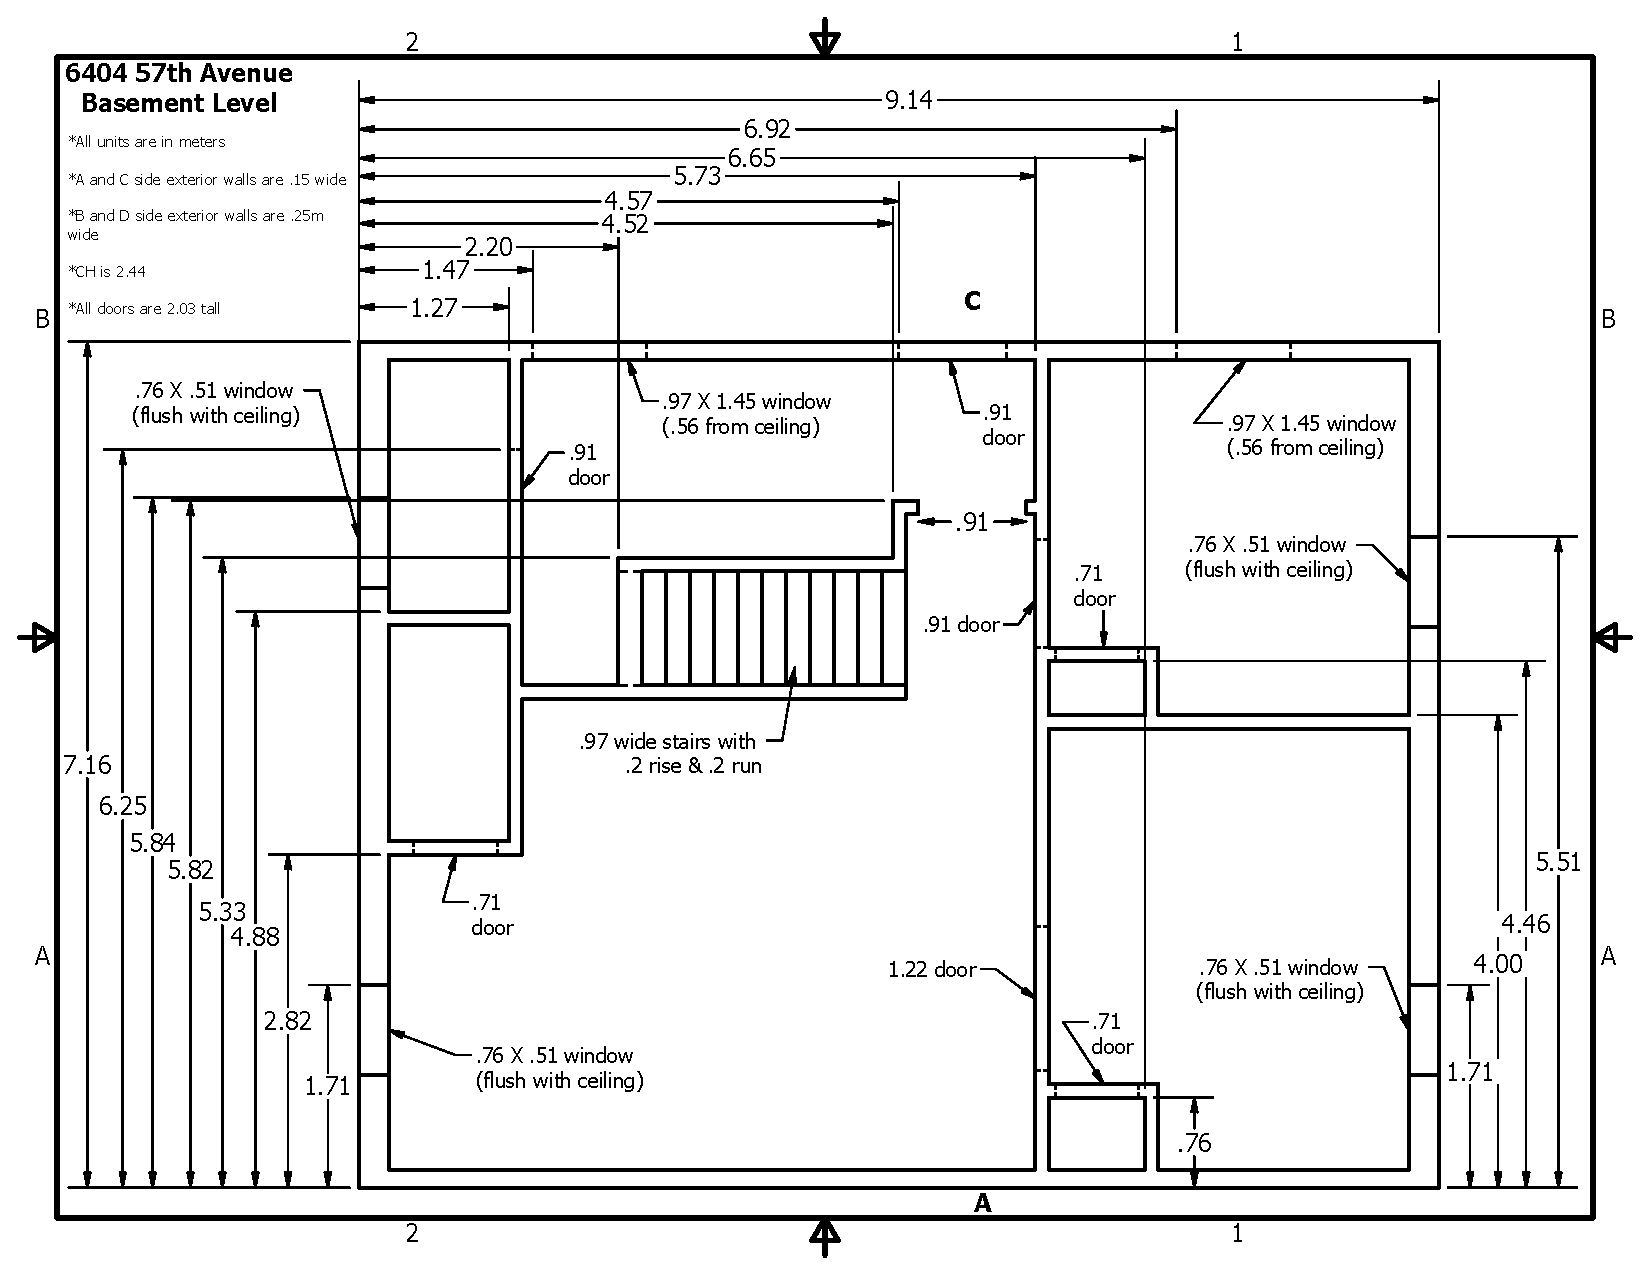
\includegraphics[width=1\textwidth]{../Figures/Basement_Metric}
\caption[Dimensioned drawing of first floor.]{Dimensioned drawing of the basement. The measurements are accurate to within 15~cm (6~in).}
\label{fig:first_floor}
\end{figure}

\begin{figure}[!ht]
\centering
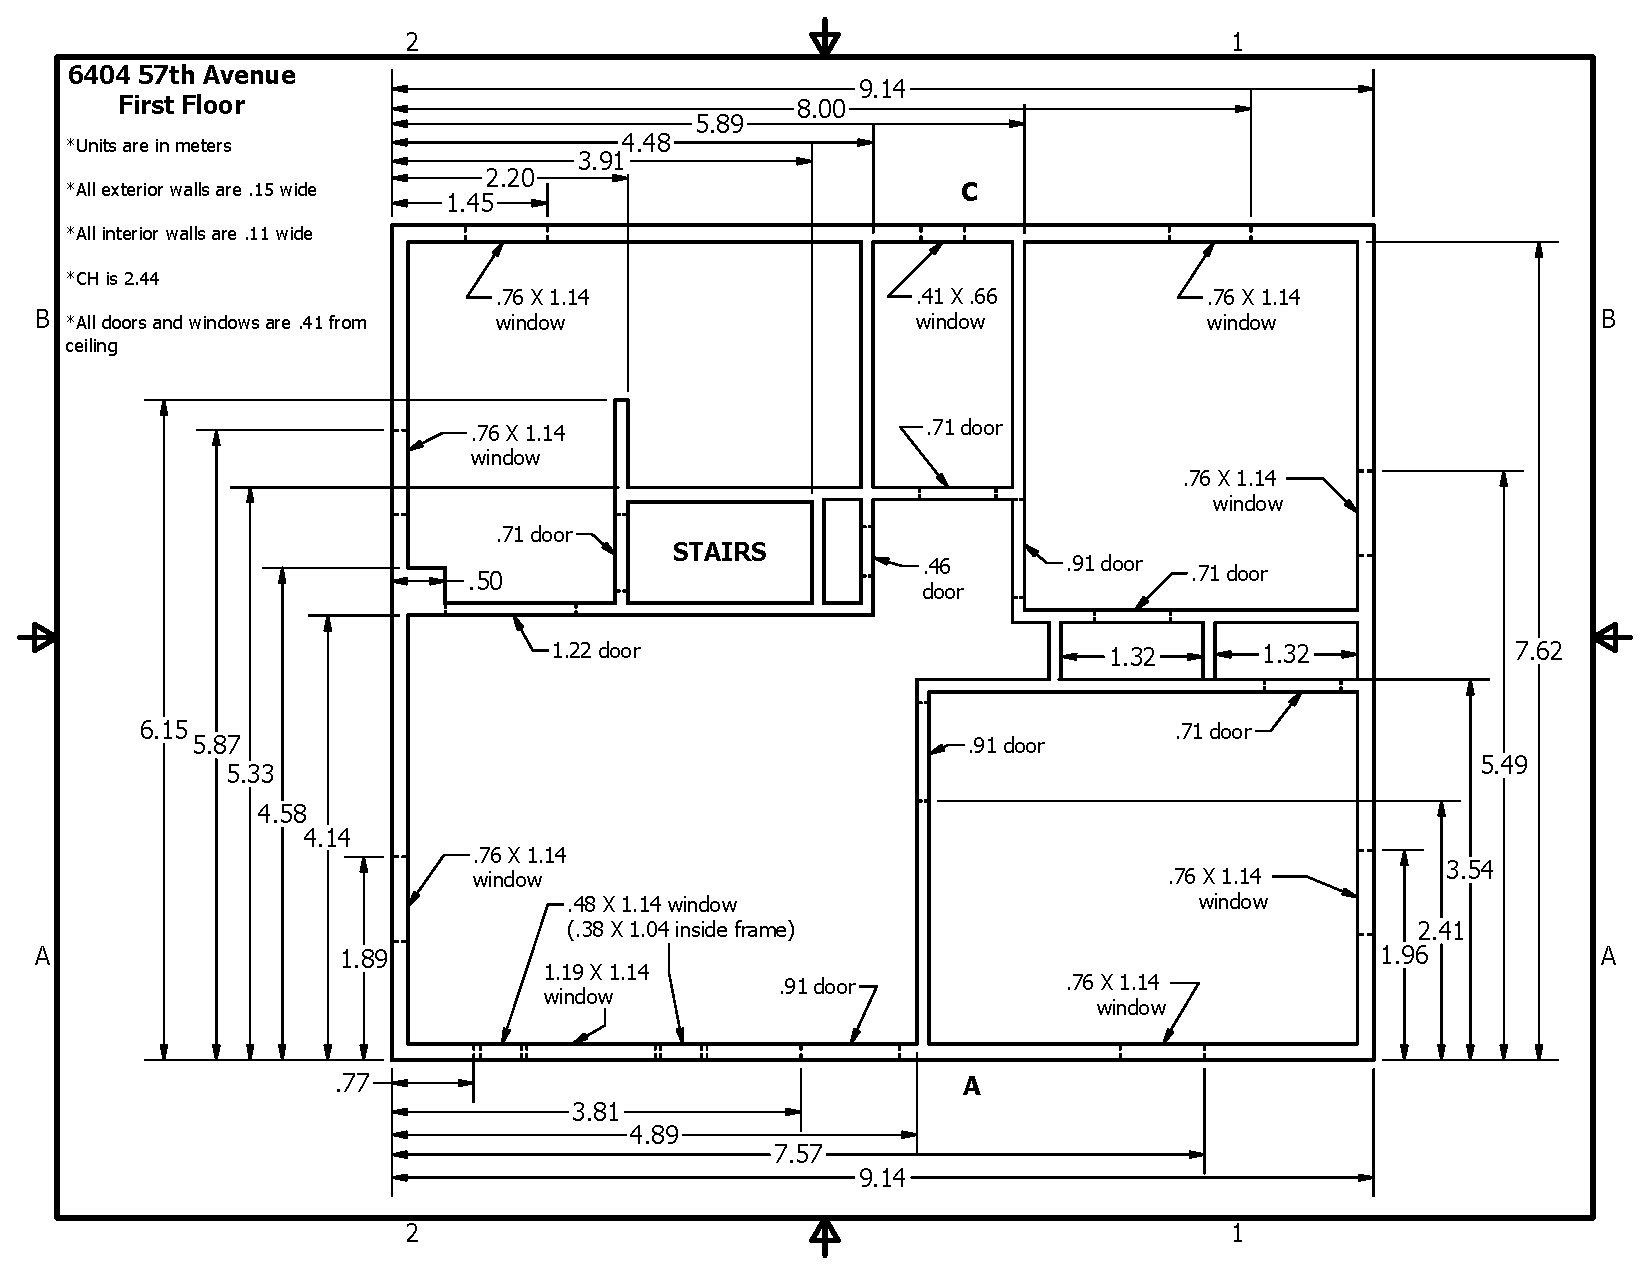
\includegraphics[width=1\textwidth]{../Figures/First_Floor_Metric}
\caption[Dimensioned drawing of second floor.]{Dimensioned drawing of the first floor. The measurements are accurate to within 15~cm (6~in).}
\label{fig:second_floor}
\end{figure}


\end{document}
